%!TEX root = ../report.tex

\chapter{State of the Art}

%\section{Deep neural network}
%From wikipedia \cite{wikidnn} deep neural networks (DNN) are type of artificial neural networks which can have many layers between their input and output. The DNN can be used to estimate the underlying mathematical manipulation
%which maps the output to the input in, a manner which is more of less consistent across all the samples. The network calculate for all the layers the probability of each outputs and then the correct label can be displayed as output 
%if the probability is above a certain threshold. Each mathematical manipulation can be considered a layer, a DNN can have many such operating layers, that is why it is named deep neural network. For example, in our scenario two sonar 
%image patches are given as input to the DNN, it will calculate different features from both image patches and at the end it will decide if the derived features are similar then the input patches are similar.

\section{Convolutional Neural Network}
Before starting with the state of the art, little introduction to the Convolutional neural network (CNN) is provided here. CNN \cite{wikicnn} is a special type of Artificial Neural Network with Multi-Layer Perceptrons (MLP),
consisting of learnable weights and biases. CNNs are usually trained with back propagation algorithm in a 
supervised manner. While a end-to-end CNN also expresses a single differentiable score function similar to a normal ANN, CNNs are different in architecture though, specially designed for recognizing visual patterns directly 
from the raw image pixels with minimal preprocessing \cite{lecun2015lenet}. Unlike fully-connected architecture, in CNN, neurons in a layer will only be connected to a small region of the layer before.
CNNs take advantage of the explicit assumption that inputs are images, as a result they can be more efficiently encoded to have much lesser parameters. The main building blocks of CNNs are Convolutional Layer (Conv), 
Pooling Layer, Fully-Connected Layer (FC). Now a typical example of a CNN can be denoted by \code{[Input - Conv - ReLU - MP - FC]}, where \code{Input} holds raw pixel values of the input image, \code{Conv} layer applies 
convolution operation to the local region of input and produce output; this operation is inspired by the natural response of a neuron in visual cortex getting stimulated. \code{ReLU} layer provides activation to each elements 
and applies a threshold (\code{max(0,x)}) so that the negative weights become zero. \code{Pooling} layer which basically down-samples the input along the spatial dimensions of supplied height and width, by mapping a cluster of neurons
from one layer to a single output in the next layer. \code{MP} or max-Pooling layer takes the maximum value from the cluster of the neurons and maps in the next layer. \code{Average} pooling takes average values of the cluster and maps to the 
next layer. Pooling can also be local or global. Lastly the \code{FC} layer just connects every neurons of one layer to the next layer, just like MLP. Fully-Connected layers serve as the decision network and determines the overall output size.
%Describe the parts of the conv net and the roles of the layers. Such as fully connected layers, max pooling, average pooling, activation functions such as Relu and Sigmoid. Initializers ?

Inspired by \cite{stateoftheart} following notation for CNN layers are used to describe components of the architectures: \code{Conv(Nf,Fw x Fh)} is a convolutional layers with Nf filters of width Fw and height Fh.
A max-pooling layer is represented by \code{MP(Pw, Ph)} where \code{Pw x Ph} is the sub-sampling size of the layer, and FC(n) is a fully connected layers where n represents output size.\\

In the following section Siamese network is briefly discussed because it is important to have a understanding of it before some of the state of the art network architectures can be explained in details. 

\section{Siamese Network}
In 1993 the concept of a new artificial neural network called Siamese network (the network in right in figure \ref{fig:two_channel_only_siamese}) was introduced by Bromley et al. \cite{bromley1994signature}. Siamese network consists two identical sub-networks which are joined at the output.
During training stage one input each is connected to each of the subnetworks. The main idea here is that the subnetworks (also called branches) are trained simultaneously and extract features from the inputs.
While the shared neurons are capable of measuring the distance between the two extracted feature vectors by each branch. If the predicted distance between two feature vectors is lesser than a threshold then it can be considered 
that the inputs are similar. Authors used this concept to compare two signatures in \cite{bromley1994signature}. One of the signature was previously obtained from the authentic owner (up to 6 signatures were recorded). This was then used to compare with a new signature
to verify if the both persons are same or not, as precaution against forgery. Authors implemented the Siamese network to be able to extract and compare different features of the two signatures and if the output is within a threshold then
they were considered matching. If not then it was most likely a forgery. 

\section{Sonar image matching techniques}

Sonar image patch matching is more difficult than normal optical patch matching problem. This is because sonar images have additional challenges such as, non-uniform insonification, low signal-to-noise ratio, poor contrast, low resolution,
low feature repeatability \cite{hurtos2013automatic} etc. But sonar image matching has important applications like in sonar registration, mosaicing \cite{kim2005mosaicing}, \cite{hurtos2012fourier} and mapping of seabed surface \cite{negahdaripour2011dynamic} etc. 
While Kim et al. \cite{kim2005mosaicing} used Harris corner detection and matched keypoints to register sonar images, Hurtos et al. \cite{hurtos2012fourier} incorporated Fourier-based features for registration of FLS images. S. Negahdaripour
et al. \cite{negahdaripour2011dynamic} estimated mathematical models from the dynamics of object movements and it's shadows. Vandrish et al. \cite{vandrish2011side} used SIFT \cite{lowe2004distinctive} for sidescan sonar image registration.
Even though these approaches did achieve considerable success in respective goals, those were found to be most effective when the rotation/translation between the frames of sonar images are comparatively smaller. Block-matching was performed 
on segmented sonar images by Pham et al. \cite{pham2013guided}, Self-Organizing Map was used for the registration and mosaicing task using sidescan sonar images. Recently, \cite{zbontar2016stereo} for stereo matching, \cite{kim2016convolutional}
for fast under-water object detection and localization, \cite{valdenegro2016objectness} objectness scoring, CNNs are being more and more used for sonar image processing. The main reason behind such rise of CNN usage is that, the CNNs can learn 
sonar-specific information from the sonar data directly. No complex manual feature design or rigorous data preprocessing steps are needed, which makes the task less complex but prediction accuracy achieved is higher.


\begin{figure}[ht]
\centering
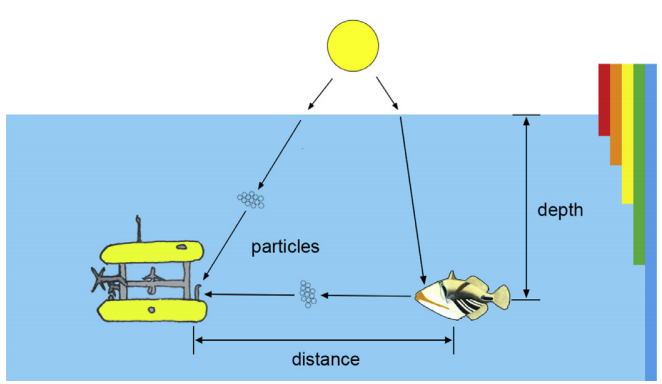
\includegraphics[width=10cm,height=5cm]{images/densenet/siamese/sonar_diagram}
\caption{Figure is taken from S. Emberton et al. \cite{emberton2018underwater}. Light gets absorbed and scattered by the particles and objects in the water, which causes poor contrast and spectral distortion in sonar images.}
\label{fig:sonar_diagram}
\end{figure}

\section{Learning similarity function}

Zagoruyko et al. have demonstrated that CNNs can be directly deployed to learn the underlying similarity function to be able to determine that two input images/patches are different instances of same object or not, 
without any help from hand designed features. The scarcity of accurate hand designed features for sonar images motivated Valdenegro et al. to evaluate similar approach as Zagoruyko et al. and encode a CNN for sonar image comparison.

Valdenegro et al. \cite{stateoftheart} evaluated two architectures, a two-channel network and a Siamese network. The architectures \ref{fig:two_channel_only_siamese} were based on the work from Zagoruyko et al. \cite{zagoruyko2015learning}.
A grid search was used over pre-defined set of parameters which define the network structure. The final two channel network structure presented in the paper for predicting binary classification score was as follows,
\code{Conv(16, 5 x 5)-MP(2, 2)-Conv(32, 5 x 5)-MP(2, 2)-Conv(32, 5 x 5)-MP(2, 2)- Conv(16, 5 x \\5)-MP(2, 2)-FC(64)-FC(32)-FC(1)}. Similarly grid search was also conducted for Siamese network structure for classification score. 
The structure for each 
of the branches or sub-network is as follows, \code{Conv(16, 5 x 5)-MP(2, 2)-Conv(32, 5 x 5)- MP(2, 2)-Conv(64, 5 x 5)-MP(2, 2)-Conv(32, 5 x 5)-MP(2, 2)\\-FC(96)-FC(96)}. The output features from the branches were then concatenated to form 192 
element vector. This was then passed through a decision network with \code{FC(64)-FC(1)}. For both two channel and Siamese network the final \code{FC(1)} layer had Sigmoid \cite{kerassigmoid} activation function and binary cross entropy loss 
\cite{kerascrossentropy} function. 

Not very complex network structures were used. In general sense, adding more layers in the network does add more non-linearity to it and in some cases, that improves the performance of the network. So in theory, more advanced networks or loss 
functions which help extracting more discriminative and patch invariant features, should improve the results even further.

\begin{figure}[ht]
\centering
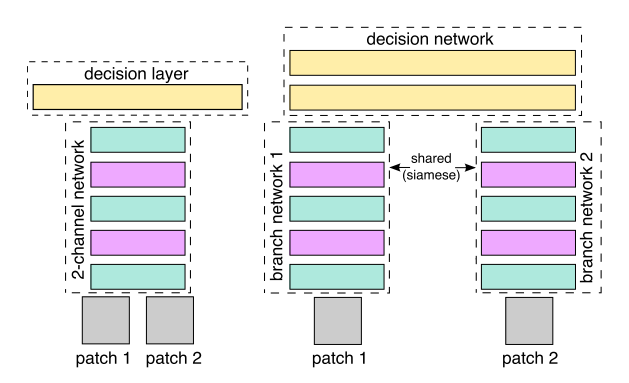
\includegraphics[height=6cm]{images/densenet/two_channel_only_siamese.png}
\caption{Two channel network (left) and Siamese (right) CNN architectures used in Valdenegro et al., though the figure and inspiration is from \cite{zagoruyko2015learning}}
\label{fig:two_channel_only_siamese}
\end{figure}
